\documentclass{beamer}

\usetheme{Goettingen}

\usepackage{amsmath}
\usepackage{enumitem}
\usepackage[T1]{fontenc}
\def\MM#1{\boldsymbol{#1}}

\newenvironment{packed_itemize}{
\begin{itemize}[leftmargin=0.1in]
  \setlength{\itemsep}{1pt}
  \setlength{\parskip}{0pt}
  \setlength{\parsep}{0pt}
}{\end{itemize}}

\title{Exascale algorithms for numerical weather and climate prediction}
\author{Jemma Shipton}
\date{9th May 2025}

\begin{document}

\begin{frame}
  \titlepage
\end{frame}

\section{Computing}
\begin{frame}{Scientific computing}
  \begin{exampleblock}{}
    \onslide<2-> \tiny {Scientific Computing is the collection of tools,
      techniques, and theories required to solve on a computer
      mathematical models of problems in Science and Engineering.  A
      majority of these tools, techniques, and theories originally
      developed in Mathematics, many of them having their genesis long
      before the advent of electronic computers. This set of
      mathematical theories and techniques is called Numerical
      Analysis (or Numerical Mathematics) and constitutes a major part
      of scientific computing. The development of the electronic
      computer, however, signaled a new era in the approach to the
      solution of scientific problems. Many of the numerical methods
      that had been developed for the purpose of hand calculation
      (including the use of desk calculators for the actual
      arithmetic) had to be revised and sometimes
      abandoned. Considerations that were irrelevant or unimportant
      for hand calculation now became of utmost importance for the
      efficient and correct use of a large Computer System. Many of
      these considerations – programming languages, operating systems,
      management of large quantities of data, correctness of programs
      – were subsumed under the new discipline of Computer Science, on
      which scientific computing now depends heavily. But mathematics
      itself continues to play a major role in scientific computing:
      it provides the language of the mathematical models that are to
      be solved and information about the suitability of a model (Does
      it have a solution? Is the solution unique?) and it provides the
      theoretical foundation for the numerical methods and,
      increasingly, many of the tools from computer science.  In
      summary, then, scientific computing draws on mathematics and
      computer science to develop the best way to use computer systems
      to solve problems from science and engineering.}
  \end{exampleblock}
  \small Gene H. Golub and James M. Ortega. Scientific Computing and Differential Equations – An Introduction to Numerical Methods. Academic Press, 1992
\end{frame}

\begin{frame}{Scientific computing}
  \small
  \begin{itemize}
    \onslide<1->\item[o] Scientific Computing is the collection of tools,
    techniques, and theories required to solve on a computer
    mathematical models of problems in Science and Engineering.
    \onslide<2->\item[o] The development of the electronic computer
    signaled a new era in the approach to the solution of scientific
    problems.
    \onslide<3->\item[o] Considerations that were irrelevant
    or unimportant for hand calculation now became of utmost
    importance for the efficient and correct use of a large Computer
    System.
    \onslide<4->\item[o] Many of these considerations –
    programming languages, operating systems, management of large
    quantities of data, correctness of programs – were subsumed under
    the new discipline of Computer Science.
    \onslide<5->\item[o]
    \textit{But mathematics continues to play a major role in
      scientific computing: it provides the language of the
      mathematical models that are to be solved and information about
      the suitability of a model and it provides the theoretical
      foundation for the numerical methods and, increasingly, many of
      the tools from computer science.}
  \end{itemize}
  
\end{frame}

\begin{frame}{Exascale Computing}
  \onslide<2->\centerline{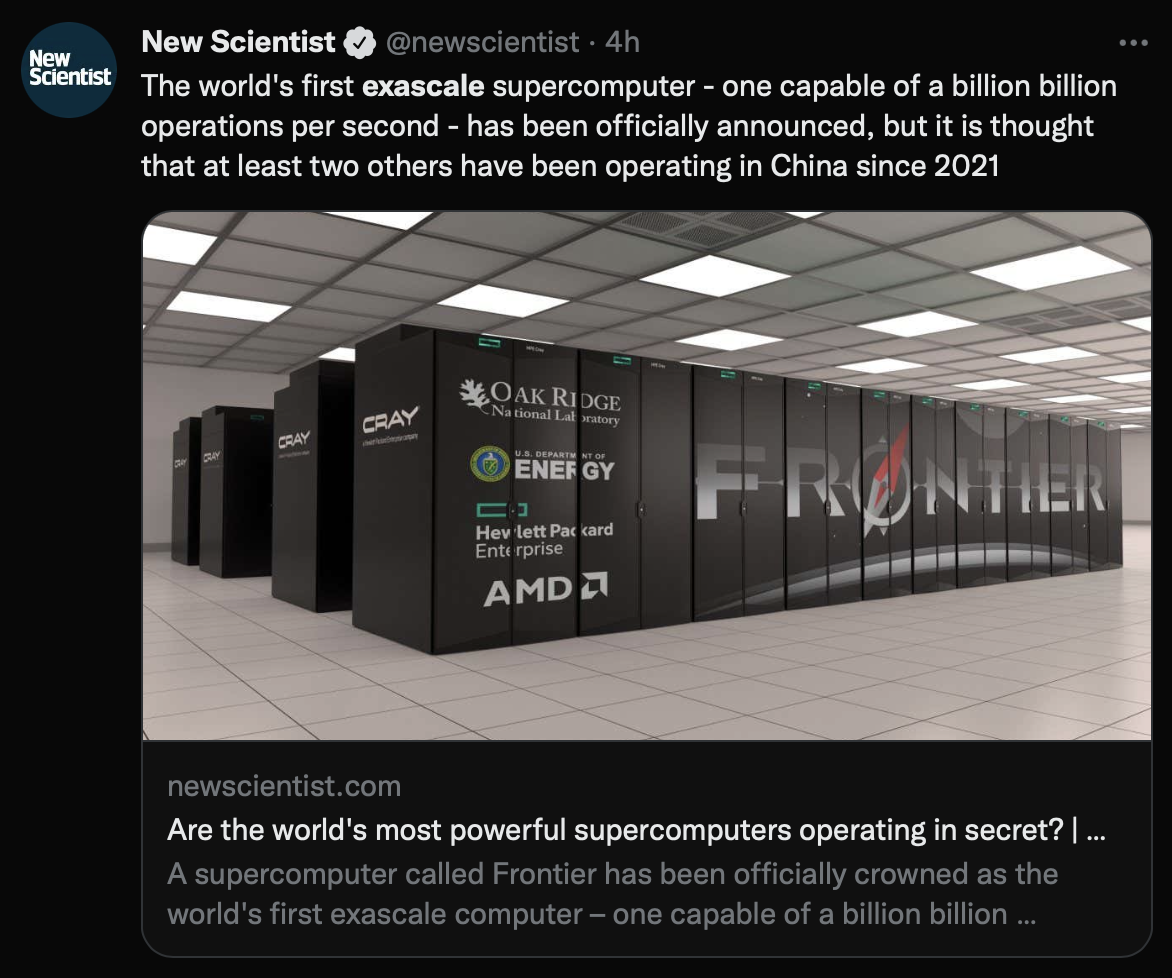
\includegraphics[width=0.85\textwidth]{figures/Frontier}}
\end{frame}

\begin{frame}{Exascale Computing}
  \centerline{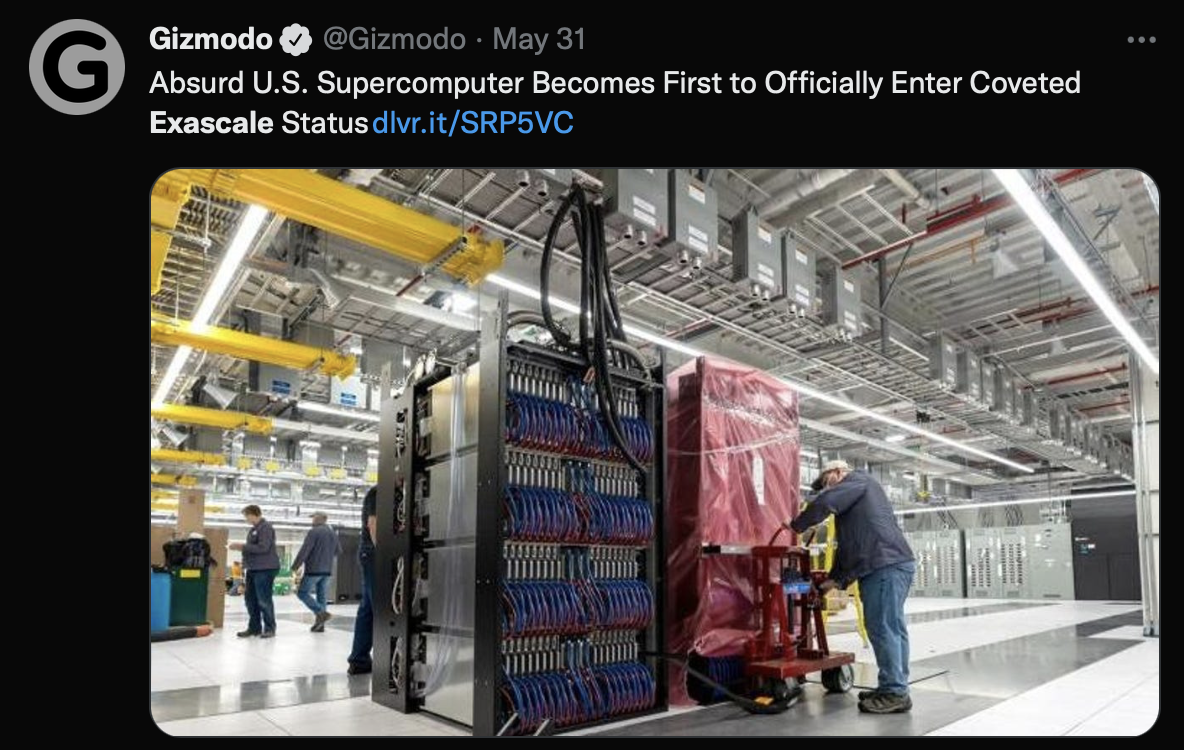
\includegraphics[width=0.85\textwidth]{figures/Frontier2}}
\end{frame}

\begin{frame}{Exascale Computing}
  \begin{itemize}
    \item[o] Trends in processor manufacture mean that we no longer
      get faster simulations by adding more of the same types of
      components.
    \item[o] There is no such thing as a `standard' exascale computer
      - processors are becoming more specialised.
    \item[o] The computer processor market is not driven by scientific
      applications.
    \item[o] Very high levels of parallelism (or `concurrency') are required.
    \item[o] Arithmetic is cheap and data movement is expensive -
      especially accessing data off-node. Communication of data slows
      down the calculation.
  \end{itemize}
   N. Thompson, S. Spanuth, The Decline of Computers as a General Purpose Technology, Commun ACM 2
\end{frame}

\section{Algorithms}
\begin{frame}{Numerical weather and climate prediction}
  \begin{columns}[T]
    \begin{column}{0.33\textwidth}
      \centerline{Observations}
      \vspace{0.2cm}
      \centerline{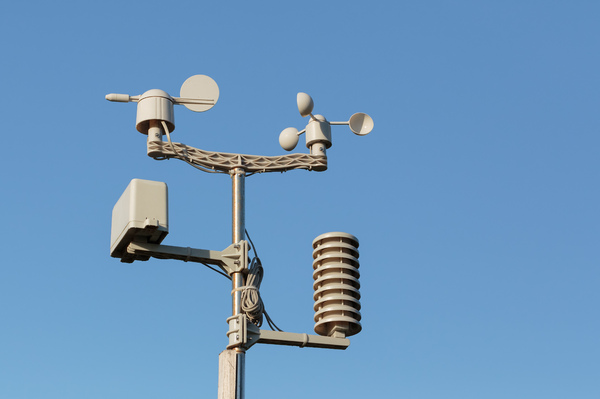
\includegraphics[width=\columnwidth]{figures/obs.jpg}}
    \end{column}
    \begin{column}{0.33\textwidth}
      \centerline{Simulation}
      \vspace{0.2cm}
      \centerline{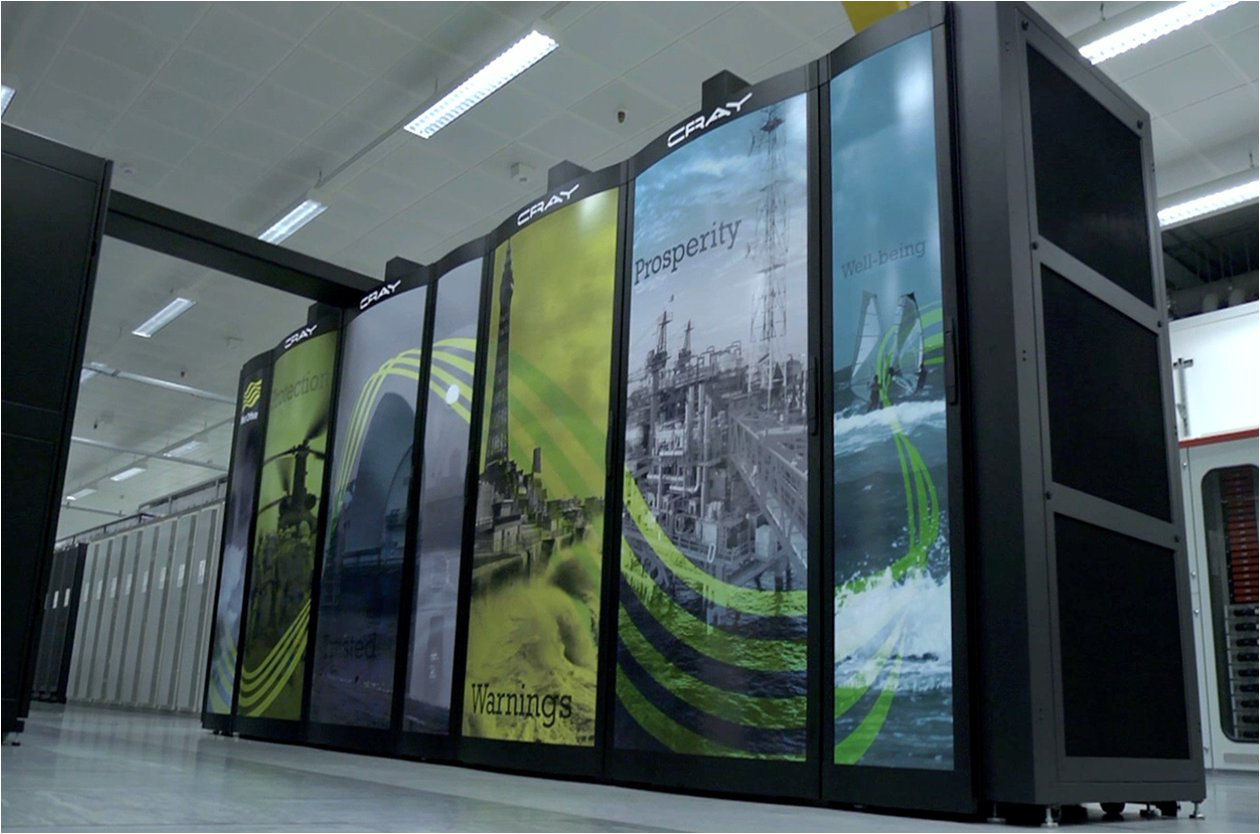
\includegraphics[width=\columnwidth]{figures/MOCray}}
    \end{column}
    \begin{column}{0.33\textwidth}
      \centerline{Forecast}
      \vspace{0.2cm}
      \centerline{
\includegraphics[width=\columnwidth]{figures/mini_forecast2.png}}
    \end{column}
  \end{columns}
  \vspace{1cm}
  \onslide<2->\begin{block}{Dynamical core}
  \vspace{-0.5cm}
    \begin{align*}
      \MM{u}_t + (\MM{u}\cdot\nabla)\MM{u} + 2\MM{\Omega}\times\MM{u} + c_p\theta\nabla\Pi + g\MM{k} &= 0, \\
      \rho_t + \nabla\cdot(\rho\MM{u}) &= 0, \\
      \theta_t + (\MM{u}\cdot\nabla)\theta &= 0.
    \end{align*}
  \end{block}
\end{frame}

\begin{frame}{How to solve a PDE on a (super)computer}
  \begin{minipage}{0.65\textwidth}
    \small
    \begin{packed_itemize}
    \item[] Solve $\MM{U}_t + \mathcal{F}(\MM{U}) = 0$ given $\MM{U}(0) =
    \MM{U}_0$.
    \onslide<2->\item[]Represent spatial derivatives on a grid.
    \onslide<3->\item[]Step forward in time calculating \\$\MM{U}_{n+1} = \mathcal{T}(\MM{U}_n)$.
    \end{packed_itemize}
  \end{minipage}
  \begin{minipage}{0.3\textwidth}
    \vspace{0.1cm}
    \onslide<2->\centerline{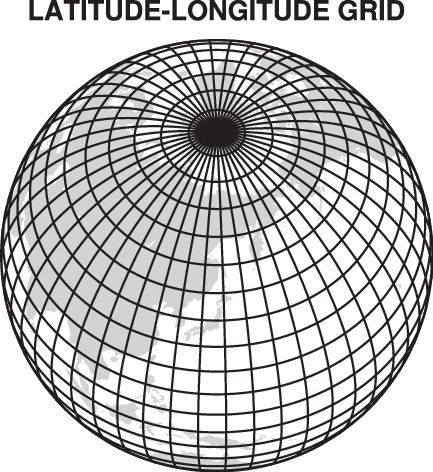
\includegraphics[width=0.95\textwidth]{figures/latlon.png}}
  \end{minipage}
  \onslide<4->Where's the parallelism? \\ \onslide<5->Spatial domain decomposition.
  \onslide<5->\centerline{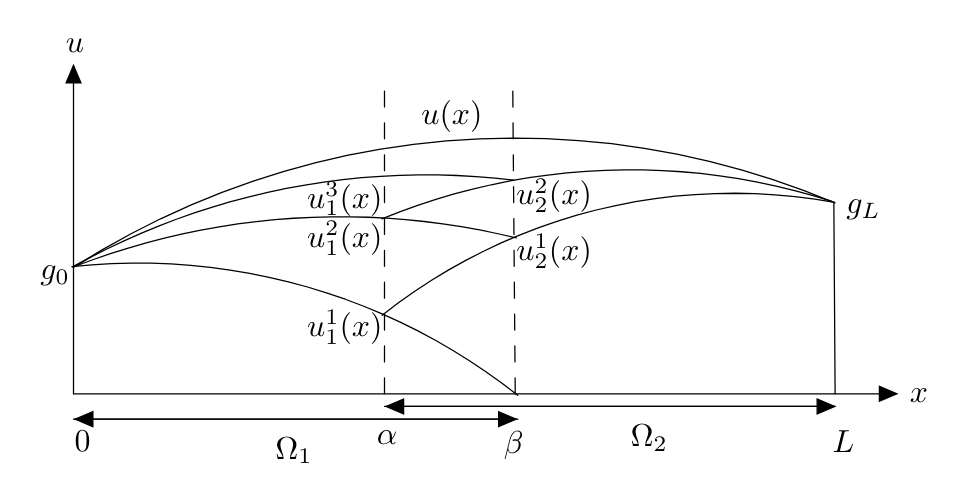
\includegraphics[width=0.95\textwidth]{figures/DD.png}}
\end{frame}

\begin{frame}{Changes to algorithms driven by parallelism}
  \centerline{\onslide<1->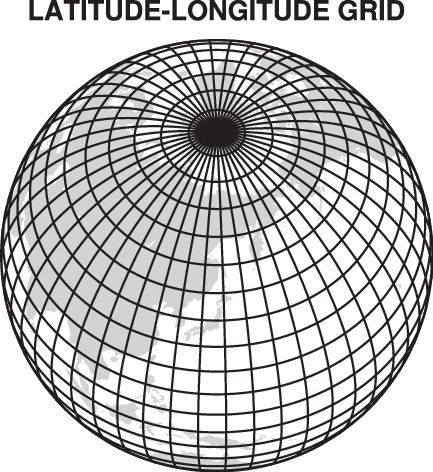
\includegraphics[width=0.32\textwidth]{figures/latlon.png}\hfill\onslide<5->
\includegraphics[width=0.32\textwidth]{figures/cs.png}\hfill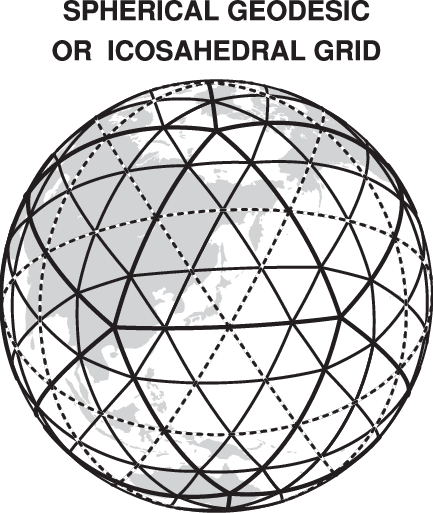
\includegraphics[width=0.32\textwidth]{figures/icos.png}}
  \onslide<2->\begin{block}{Challenge: bottleneck due to data communication}
  \begin{itemize}[leftmargin=0.1in]
    \small
    \onslide<3->\item \textbf{Strong scaling:} more processors leads to more communication
    \onslide<4->\item \textbf{Weak scaling:} increase problem size, e.g. increase resolution... but then we have to decrease the timestep
    \end{itemize}
  \end{block}
  \onslide<5->One solution: use a different grid... and then a different algorithm.
  
\end{frame}

\begin{frame}{Changes to algorithms driven by parallelism}

  \vspace{0.1cm}
  \includegraphics<1>[width=0.85\textwidth]{figures/Parareal_Figs/Parareal1.png}%
  \includegraphics<2>[width=0.85\textwidth]{figures/Parareal_Figs/Parareal2.png}%
  \includegraphics<3>[width=0.85\textwidth]{figures/Parareal_Figs/Parareal3.png}%
  \includegraphics<4>[width=0.85\textwidth]{figures/Parareal_Figs/Parareal4.png}%
  \includegraphics<5>[width=0.85\textwidth]{figures/Parareal_Figs/Parareal5.png}%
  \includegraphics<6>[width=0.85\textwidth]{figures/Parareal_Figs/Parareal6.png}%
  
  \onslide<2->\begin{block}{}
    We partition the time domain into intervals and use $G$ to give us
    an initial condition for $F$ on each interval.
  \end{block}
  \vspace{-5mm}
  \onslide<3->\begin{block}{}
    $F$ can be computed in parallel, although the later time intervals
    do not have an accurate initial condition.
  \end{block}
  \vspace{-5mm}
  \onslide<4->\begin{block}{}
    We iterate, correcting the initial condition on each interval:
    \begin{align*}
      u_0^{k+1} &= u^0 \\
      u_{n+1}^{k+1} &= F(u_n^k) + G(u_n^{k+1}) - G(u_n^k)
    \end{align*}
  \end{block}
\end{frame}

\begin{frame}{Changes to algorithms driven by parallelism}

  \begin{block}{Challenge: We're using more processors but do we get the solution any quicker?!}
    \begin{packed_itemize}
    \item $G$ must be cheap to evaluate as it is the serial bottleneck in the simulation.
    \item $G$ must be accurate enough that information is communicated to later time slices, enabling fast convergence.
    \end{packed_itemize}
  \end{block}
\end{frame}

\section{New frontiers in research}
\begin{frame}{New frontiers in research}
  \begin{itemize}
    \item[o] `Paradigm shift' in algorithm development due to hardware changes.
    \item[o] Convergence of parallel-in-time algorithms is problem specific and the choice of algorithm will depend on the problem.
    \item[o] Multiscale problems (e.g. adding `physics' to `dynamics')
    \item[o] What are good test problems? How do we know our code is right?
    \item[o] What trade offs can be made to optimise a particular problem on a particular architecture?
    \item[o] Where does machine learning fit in with algorithm development?
  \end{itemize}
\end{frame}

\begin{frame}{What are the practical implications?}
  \begin{itemize}
  \item[o] `Separation of concerns': algorithm implementation separate from parallelisation.
  \item[o] Flexible software is required for rapid prototyping of new algorithms.
  \item[o] Software becomes complex with a large `stack' of dependencies.
  \item[o] Performance modelling is really hard - sometimes the only way to find out is to run the code.
  \item[o] Access to HPC is really important.
  \item[o] Well-qualified people are \textbf{\emph{absolutely essential}} for accessing HPC and building the software.
  \item[o] Communication between domain scientists, algorithm developers and software/hardware analysts is crucial (and fun!)
  \end{itemize}
  \url{https://www.metoffice.gov.uk/research/approach/modelling-systems/lfric}
\end{frame}


\end{document}
